% This is "sig-alternate.tex" V1.8 June 2007
% This file should be compiled with V2.3 of "sig-alternate.cls" June 2007
%
% This example file demonstrates the use of the 'sig-alternate.cls'
% V2.3 LaTeX2e document class file. It is for those submitting
% articles to ACM Conference Proceedings WHO DO NOT WISH TO
% STRICTLY ADHERE TO THE SIGS (PUBS-BOARD-ENDORSED) STYLE.
% The 'sig-alternate.cls' file will produce a similar-looking,
% albeit, 'tighter' paper resulting in, invariably, fewer pages.
%
% ----------------------------------------------------------------------------------------------------------------
% This .tex file (and associated .cls V2.3) produces:
%       1) The Permission Statement
%       2) The Conference (location) Info information
%       3) The Copyright Line with ACM data
%       4) NO page numbers
%
% as against the acm_proc_article-sp.cls file which
% DOES NOT produce 1) thru' 3) above.
%
% Using 'sig-alternate.cls' you have control, however, from within
% the source .tex file, over both the CopyrightYear
% (defaulted to 200X) and the ACM Copyright Data
% (defaulted to X-XXXXX-XX-X/XX/XX).
% e.g.
% \CopyrightYear{2007} will cause 2007 to appear in the copyright line.
% \crdata{0-12345-67-8/90/12} will cause 0-12345-67-8/90/12 to appear in the copyright line.
%
% ---------------------------------------------------------------------------------------------------------------
% This .tex source is an example which *does* use
% the .bib file (from which the .bbl file % is produced).
% REMEMBER HOWEVER: After having produced the .bbl file,
% and prior to final submission, you *NEED* to 'insert'
% your .bbl file into your source .tex file so as to provide
% ONE 'self-contained' source file.
%
% ================= IF YOU HAVE QUESTIONS =======================
% Questions regarding the SIGS styles, SIGS policies and
% procedures, Conferences etc. should be sent to
% Adrienne Griscti (griscti@acm.org)
%
% Technical questions _only_ to
% Gerald Murray (murray@acm.org)
% ===============================================================
%
% For tracking purposes - this is V1.8 - June 2007

\documentclass{sig-alternate}

% force letter size (default is A4)
\pdfpagewidth=8.5in
\pdfpageheight=11in

\usepackage{graphicx}

% from http://mintaka.sdsu.edu/GF/bibliog/latex/floats.html
% Alter some LaTeX defaults for better treatment of figures:
% See p.105 of "TeX Unbound" for suggested values.
% See pp. 199-200 of Lamport's "LaTeX" book for details.
%   General parameters, for ALL pages:
\renewcommand{\topfraction}{0.9}    % max fraction of floats at top
\renewcommand{\bottomfraction}{0.8} % max fraction of floats at bottom
%   Parameters for TEXT pages (not float pages):
\setcounter{topnumber}{2}
\setcounter{bottomnumber}{2}
\setcounter{totalnumber}{4}     % 2 may work better
\setcounter{dbltopnumber}{2}    % for 2-column pages
\renewcommand{\dbltopfraction}{0.9} % fit big float above 2-col. text
\renewcommand{\textfraction}{0.07}  % allow minimal text w. figs
%   Parameters for FLOAT pages (not text pages):
\renewcommand{\floatpagefraction}{0.7}  % require fuller float pages
% N.B.: floatpagefraction MUST be less than topfraction !!
\renewcommand{\dblfloatpagefraction}{0.7}   % require fuller float pages
% remember to use [htp] or [htpb] for placement
%------------------

\begin{document}
%
% --- Author Metadata here ---
\conferenceinfo{SIGCSE}{'09 Chattanooga, Tennessee, USA}
%\CopyrightYear{2007} % Allows default copyright year (200X) to be over-ridden - IF NEED BE.
%\crdata{0-12345-67-8/90/01}  % Allows default copyright data (0-89791-88-6/97/05) to be over-ridden - IF NEED BE.
% --- End of Author Metadata ---

\title{The Pintos Instructional Operating System Kernel}

% \subtitle{[Draft]}

\numberofauthors{3}
\author{
% 1st. author
\alignauthor Ben Pfaff\\
       \affaddr{Nicira Networks}\\
       \affaddr{Palo Alto, CA}\\
       \email{blp@nicira.com}
% 2nd. author
\alignauthor Anthony Romano\\
       \affaddr{Stanford University}\\
       \affaddr{Palo Alto, CA}\\
       \email{ajromano@stanford.edu}
% 3rd. author
\alignauthor Godmar Back\\
       \affaddr{Virginia Tech}\\
       \affaddr{Blacksburg}\\
       \email{gback@cs.vt.edu}
}

\maketitle
\begin{abstract}
Pintos is an instructional operating system, complete with documentation
and ready-made, structured assignments that introduce students to
the principles of multi-programming, scheduling, virtual memory,
and file systems.  By allowing students to run their work product on
actual hardware, while simultaneously benefiting from debugging
and dynamic analysis tools provided in simulated and emulated environments,
Pintos increases student engagement.  Unlike tailored versions of
commercial or open source OS such as Linux, Pintos is designed from the
ground up from an educational perspective.  
It has been used by multiple institutions for a number of years and
is available for wider use.
%Finally, Pintos includes a set of debugging, diagnosis, and dynamic analysis 
%tools to reduce the complexity of kernel-level development.

\end{abstract}

% A category with the (minimum) three required fields
%\category{H.4}{Information Systems Applications}{Miscellaneous}
%A category including the fourth, optional field follows...
%\category{D.2.8}{Software Engineering}{Metrics}[complexity measures, performance measures]

% http://www.cs.arizona.edu/groups/sigcse09/format.html#reqs suggests
\category{K.3.2}{Computers and Education}{Computer and Information Science Education}

\terms{Design, Experimentation}

\keywords{Pintos, instructional operating system, instructional kernel}

\newcommand{\pintosenvfigure}{
    \begin{figure}[htp]
    \centering
    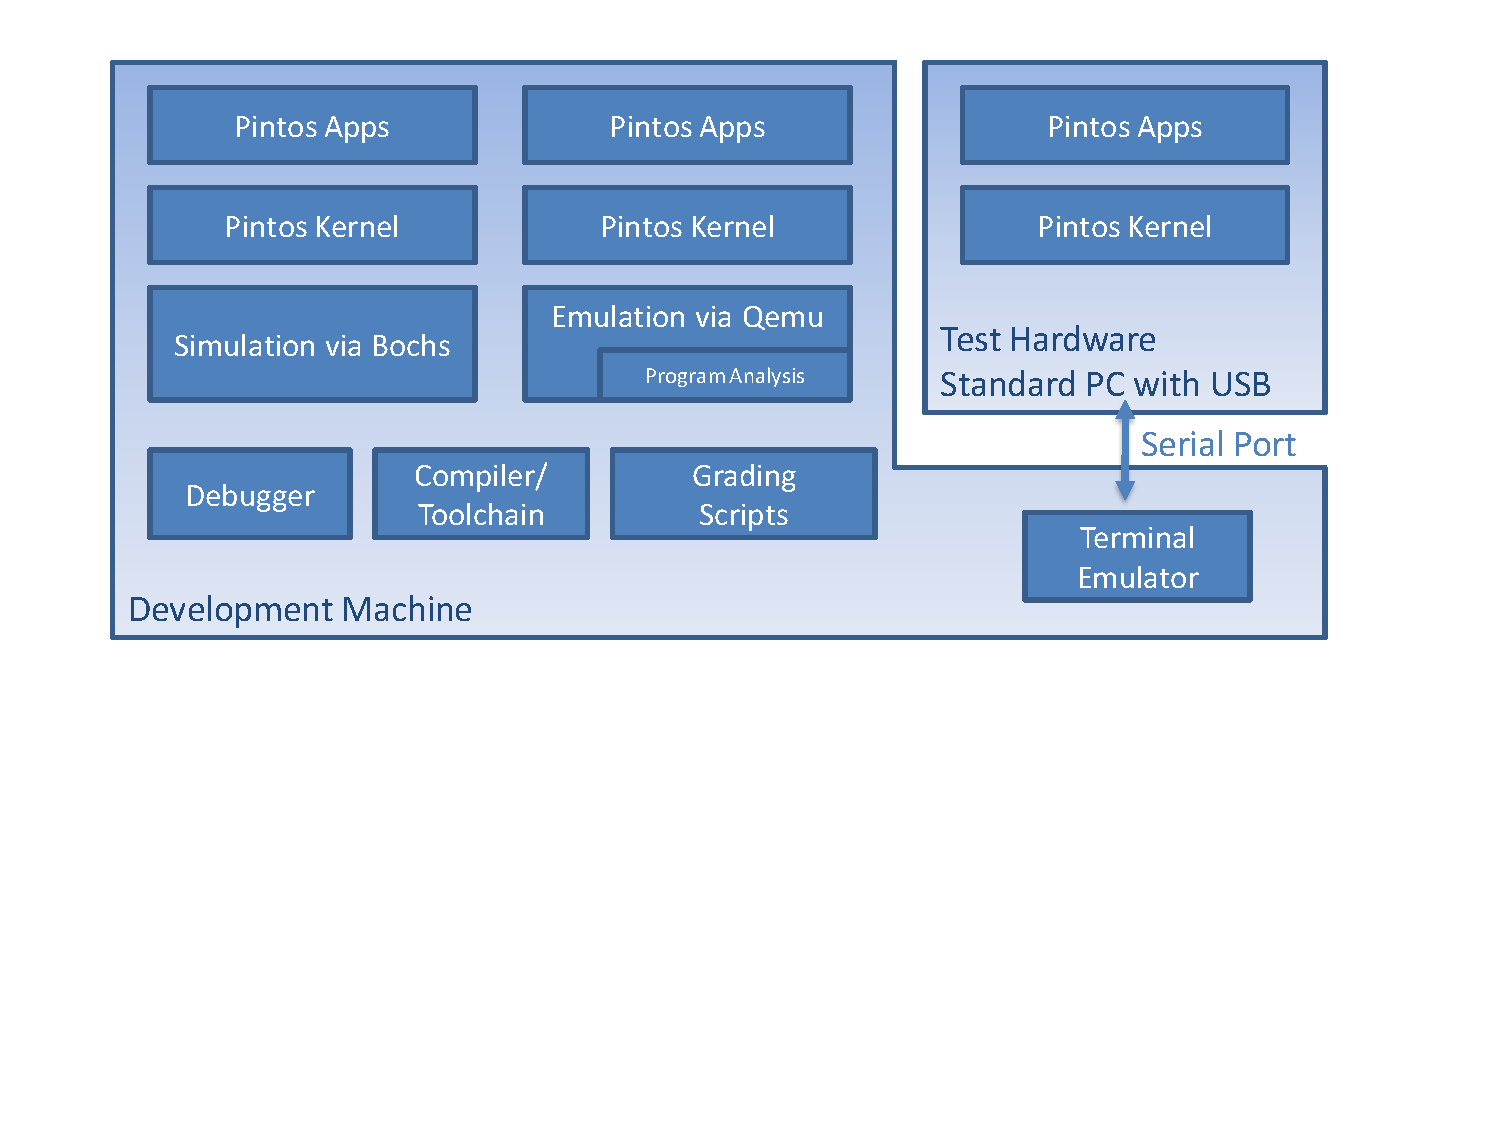
\includegraphics[trim=.5in 3.2in .7in .3in, clip,width=\columnwidth]{pintosoptions.pdf}
    \caption{The same Pintos instructional kernel runs in a
    fully reproducible simulated environment, in an enhanced
    emulated environment with dynamic analysis capability, and
    on actual hardware.}
    \label{fig:pintosenvs}
    \end{figure}
}

\newcommand{\pintosdetailfigure}{
    \begin{figure*}[htp]
    \centering
    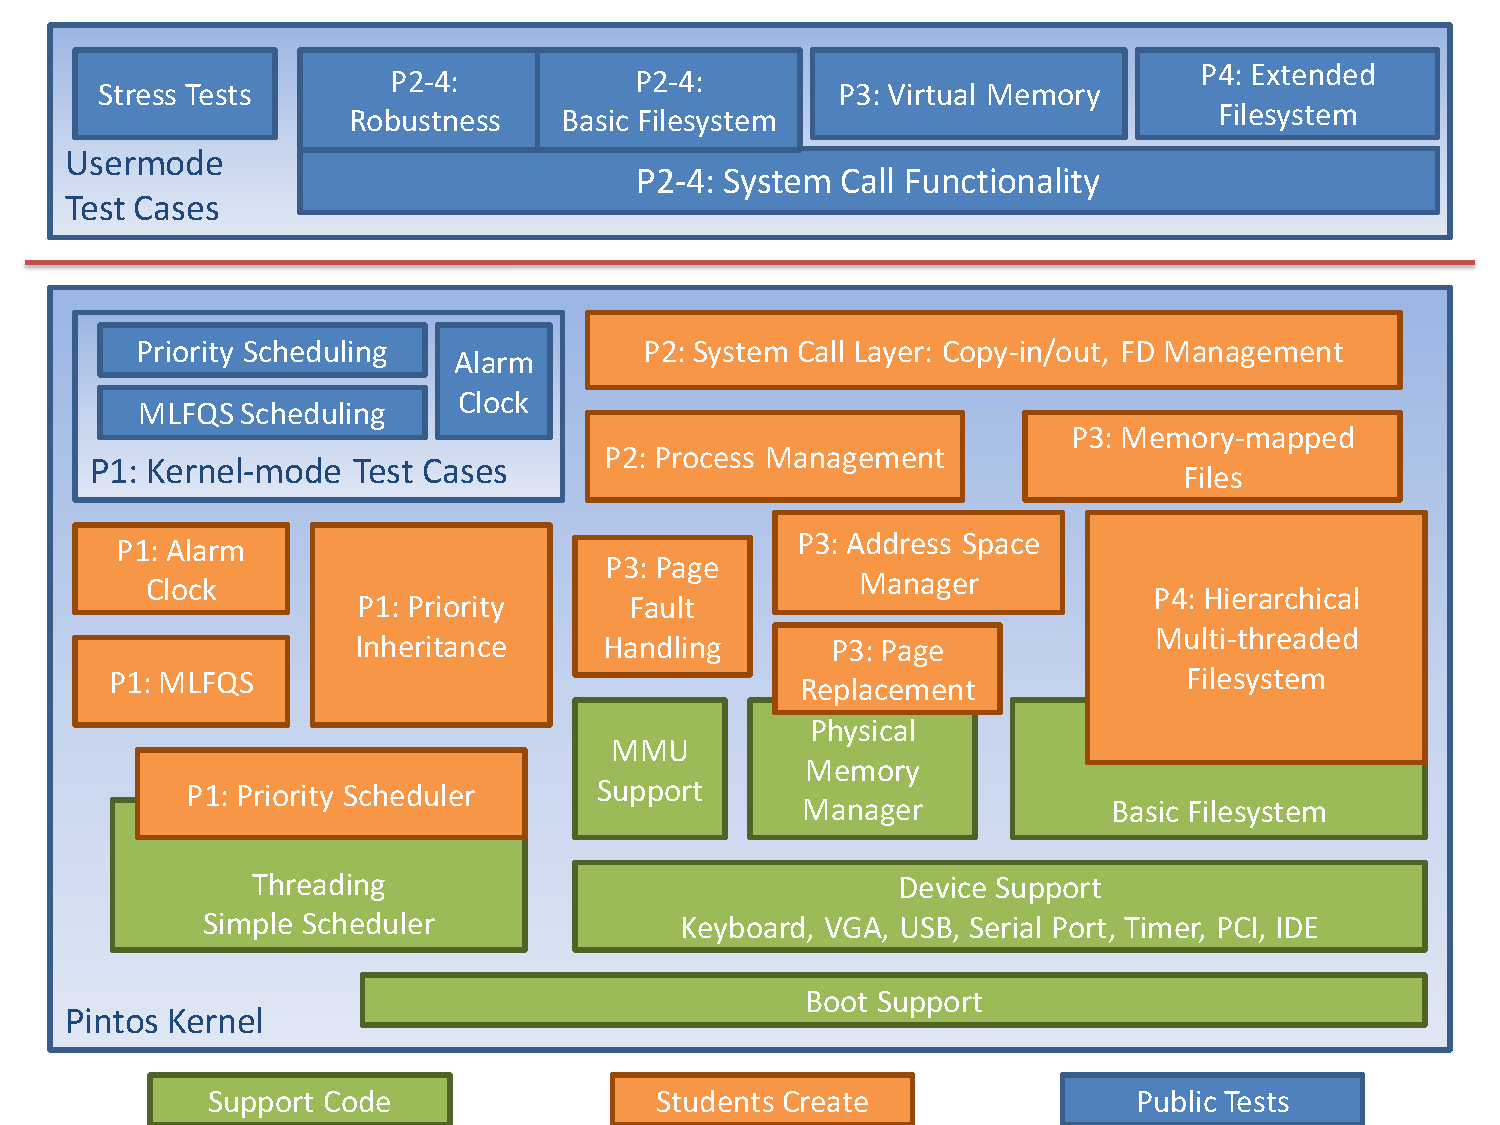
\includegraphics[width=.7\textwidth]{pintosoverview.pdf}
    \caption{Components of Pintos split in provided support code, test cases, 
        and components created in assignments.  Overlapping components indicate
        when students have to replace parts of the support code.}
    \label{fig:pintosdetail}
    \end{figure*}
}

\newcommand{\pintostestcounttable}{
\begin{table}
    \begin{tabular}{lccc}
    Project & Functionality & Robustness & Regression \\
    1       & 27            & -          & -          \\
    2       & 41            & 35         & -          \\
    3       & 20            & 14         & 75         \\
    4       & 39            & 7          & 75         \\
    \end{tabular}
    \caption{Pintos test cases by project.}
    \label{table:tests}
\end{table}
}


\section{Introduction}
\label{sec:intro}

Despite the wide use of higher-level languages and environments, gaining a robust
understanding of operating systems (OS) fundamentals and training in the current design and
implementation practices of OS remains a cornerstone goal of 
undergraduate computer science education.

% abstract/concrete
% internal/external
Approaches to teaching OS courses generally fall along two axes: 
whether the treatment of the material is abstract or 
concrete~\cite{Hovemeyer2004Running}, and whether they adopt an
internal or external perspective~\cite{Deitel2003Operating}.
An abstract approach discusses algorithms and techniques used in operating 
systems and may include partial implementation or simulation exercises,
whereas a concrete approach stresses the design and creation of 
realistic artifacts.
When adopting the internal perspective, an operating system is considered
from the point of view of the OS designer, whereas the external perspective 
assumes the role of a user or programmer using an OS's 
facilities~\cite{Bryant2002Computer}.

% is this too controversial for this audience?
The approach advocated in this paper adopts a concrete approach and the internal
perspective.  Students who have been in the role of an
OS designer bring a better understanding of how to use one; and students
who have both studied, implemented, and evaluated core OS techniques obtain 
a deeper understanding than those who have merely studied them.
Finally, adopting a concrete approach brings significant secondary
benefits, including training in modern software development techniques
and tools.  The C language remains the implementation language of choice
for operating system kernels and for many embedded systems.
Practice and debugging skills in C, particularly using modern tools,
not only increases students' ``market value,''~\cite{1292450} but provides students with
the insight that a low-level programming and runtime model is not incompatible
with high-level tools.

Designing course material for the internal and concrete 
approach is challenging for several reasons.  While realistic, 
assignments should be relatively simple and doable within a realistic time frame.  
Whereas assignments should use current hardware architectures, 
they must not impart too much transient knowledge.
Assignments should include and emphasize the use of modern software 
engineering practices and tools, such as dynamic program analysis.

This paper introduces Pintos, an instructional operating system kernel that 
has been in use at several institutions for about 4 years.  Pintos provides 
a bootable kernel for standard personal computers.  We provide several
structured assignments in which students implement a basic priority
scheduler, a multi-level feedback queue scheduler, a process-based 
multi-programming system, page-based virtual memory
including on-demand paging, memory-mapped files, and swapping, and a
simple hierarchical file system.  An overview of the projects enabled
by Pintos is given in Figure~\ref{fig:pintosdetail}, which shows which
software is provided as support code and test cases,
the parts that are created by students, and their relationship. 

Although Pintos follows in the tradition of instructional operating systems 
such as Nachos~\cite{Christopher1993Nachos}, OS/161~\cite{Holland2002New}, and
GeekOS~\cite{Hovemeyer2004Running}, 
PortOS~\cite{Atkin2002PortOS}),
BLITZ~\cite{PorterOverview},
JOS~\cite{1088822}, or Yalnix~\cite{1088822},
we believe that it is unique in two
aspects.  First, Pintos runs on both real hardware and in emulated and
simulated environments.\footnote{\small GeekOS is the only other system that claims to 
also run on real PC hardware; it requires, however, a dedicated disk and 
does not support running off USB devices, making it impractical for many 
laboratory settings.}  We believe that having the ability to see the outcome
of their project interact with actual hardware increases student engagement.
Second, we have created a set of analysis tools
for the emulated environment that allows students to detect programming
mistakes such as race conditions.  Figure~\ref{fig:pintosenvs} shows
the three environments in which the same kernel can be run.

Others have used Linux, either on dedicated devices (e.g., iPodLinux~\cite{1352199}),
or in virtualized environments~\cite{1008027,1352648,Nieh2005Experiences}, to provide
an internal, concrete perspective.  Compared to those approaches, Pintos provides
a similar level of realism to students in that they can see the result of their
work on concrete or virtualized hardware, but does not require that students 
understand the often arcane and ill-documented interfaces of the Linux kernel,
which were not designed from an educational perspective.  By contrast, all
Pintos code is written to be studied by students.

%This paper summarizes the design philosophy that underlies Pintos,
%details its structure, and outlines the nature and learning goals of each
%assignment.

\pintosenvfigure{}

\pintosdetailfiguretwo{}

% Challenges.
% How to embed principles?
% How to teach software engineering?
% Realism vs. Simplification

%User-Mode Linux\cite{1008027}
%Virtualization\cite{1352648}
%Linux in VM\cite{Nieh2005Experiences}



\section{Design Principles}
\label{sec:designprinciples}

Pintos's projects are built on a number of principles.

\paragraph{Read before you Code}
Each project involves a significant amount of reading code before
students write the first line of code.
Because software maintenance constitutes the vast majority of all
software development efforts~\cite{Boehm1981Software}, this setup mirrors the 
environment in which most software engineers work.
Simultaneously, we limit the amount students have to read
by encapsulating lower layers, such as device drivers.
We went to great lengths to write the entire Pintos baseline code,
and in particular the portions students must read, in a style that shows,
by example, the coding style we expect from students.  
% cut for length
%This style includes purely syntactical convention such as the choice of the
%GNU indentation style, and extends to commenting style and naming conventions.
We continuously refined the internal code documentation over several
semesters, focusing on those 
portions that initially proved difficult to understand or confusing.

\paragraph{Maximize Creative Freedom}
OS design involves a tremendous amount of creative freedom, both in the
choice of algorithm and data structures.  Our projects are designed to
stimulate creativity by avoiding the prescription of specific approaches
to accomplish each project's goals.  Instead, students must design their
own data structures and associated algorithms as much as possible.

\paragraph{Practice Test-driven Development}
%Test-driven development~\cite{Edwards}
Each project includes a large number of test cases that is accessible
to students, as shown in  Table~\ref{table:tests}.  
They must implement the API that is exercised by these test cases.  
Students are encouraged to add their own test cases.

\paragraph{Work in a Team}
The projects presented in this paper are designed to be accomplished by teams of 
2-4 students.  Working in a team provides an environment that more closely resembles
industrial software development, and it provides a way for students to brainstorm and
implement together.  In addition, we teach and require the use of group collaboration tools,
notably shared source code version control systems such as CVS.

\paragraph{Justify your Design}
Design justification and rationale is as important for learning as creating an artifact 
that fulfills a set of given requirements.  We designed a set of structured questionnaires 
in which students describe their design and discuss choices and trade-offs they made.

\paragraph{Provide a Reproducible, Manageable Environment}
Operating Systems are inherently concurrent environments, which can be difficult
to debug.  For educational use, we must provide an environment that is
manageable and reproducible, which we do by providing the option
of running Pintos in a simulated, fully deterministic environment.  
As a result, Pintos kernels can be debugged in a manner that
is substantially similar to how user programs are being debugged.

\paragraph{Include Analysis Tools}
Static and dynamic analysis tools are now being widely used; an OS course should
be no exception.  We have extended the QEMU emulator~\cite{Bellard2005QEMU} to 
perform tailored analyses that point out errors such as race conditions.

\paragraph{Provide Extensive and Structured Documentation}
If using an instructional system requires too much undocumented knowledge,
the system is often not shared, or falls into disuse, because the learning curve
for instructors wishing to use it is too steep and training teaching assistants is difficult.
Pintos includes an extensive 129 page manual, a sample solution,
and instructions for teaching assistants.  The assignment documentation separates sections 
students must read from sections that merely provide supplemental information.
%Even though Pintos uses an existing and complex architecture, our experience indicates
%that the manual is sufficient for most students.



\section{Assignments}
\label{sec:assignments}

\pintostestcounttable{}

%
% Not sure if we need that.
%
% \subsection{Project 0}
% If Pintos is used in a semester-long course, project 0 serves as a ``warm-up'' project.
% In this project, students will gain familiarity with the Pintos source tree and some
% supporting classes, in particular its implementation of doubly-linked lists.
% In OS, doubly-linked lists are frequently used because they allow $O(1)$ insertion and
% removal operations.  Moreover, they are often used in a style in which the list cell
% containing the next and prev pointers is embedded in some larger structure, such as
% a thread control block, rather than having separately allocated list cells.
% In project 0, students use Pintos's list implementation to implement a simple, first-fit 
% memory allocator.  

\subsection{Project 1 -- Threads}
% intro
Project 1 revolves around threads.  The baseline Pintos code boots into a kernel that
supports multiple in-kernel threads.  It provides code for initialization, thread creation and
destruction, context switches, thread blocking and unblocking as well as a simple but
preemptive round-robin scheduler.
Students study the existing, barebones threading system (about 600 lines of C code) to 
understand how threads are created and destroyed, and to understand the transitioning of 
threads between the READY, RUNNING, and BLOCKED states.  They also study how a thread's
internal memory is managed, which is used to store its runtime stack and thread control block.
Students can examine the context switch code, but the projects do not involve any modifications
to it.

After reading the baseline code, the project asks students to implement several features
that exercise thread state transitions.  The first part of this project includes a simple
alarm clock, which requires maintaining a timer queue of sleeping threads and changing 
the timer interrupt handler to unblock those threads whose wakeup time has arrived.
Students learn how to protect data structures that are shared between a thread and an
interrupt handler.  The second part of the project constitutes a strict priority-based
uniprocessor scheduler; students learn about the different ways in which 
such a scheduler must react to thread state changes.
% cut for length
%Project 1 also introduces synchronization primitives such as semaphores, locks,
%and condition variables and explores the interaction between such primitives,
%thread states, and the scheduler.

Based on the priority scheduler, students implement priority inheritance, 
which deepens their understanding of the interaction of threads and locks.
We use the example of the near-failure of the Mars PathFinder mission to motivate
the need for priority inheritance.  
Separately, students build a multi-level feedback queue scheduler on top of the strict
priority scheduler.  This scheduler adjusts threads' priorities based on a sampling  
of how much CPU time a thread has received recently.

\paragraph{Testing and Grading}
Project 1 is accompanied by 27 tests as shown in Table~\ref{table:tests}, which are 
run using the Bochs simulator by a grading script.  
Most tests are designed to test a single aspect, but some tests 
test more involved scenarios.  Most of the tests are designed to produce a deterministic 
output; the grading script will point out differences between the expected and the actual output. 
Usually, a test failure leads students to study the documented source code of the test
and understand how the expected output derives from it.

The MLFQS scheduler tests are graded differently. Since those tests rely on estimating CPU
usage, they depend on how much CPU time a specific implementation uses, which in turn depends on how
efficient it is.  We compute the expected CPU consumption values by simulation and provide an
envelope within which the output is accepted.  The envelope is large enough to allow for minor
inefficiencies, but major inefficiencies will usually lead to test failures.  Such failures
convey the importance of using efficient algorithms and data structures within a kernel,
because wasting CPU cycles in the kernel reduces the amount available to applications.

% intro
\paragraph{Learning Objectives}
Project 1 has three learning objectives.  First, students will understand how
the illusion that ``computers can do multiple things at once'' is created by a sequence
of thread state transitions and context switches.  Second, they will understand how
a simple underlying mechanism - such as priority-based scheduling - can lead to more
sophisticated scheduling policies.  Third, having seen the mechanisms a preemptive scheduler
uses to create apparent concurrency, students gain a better intuition of the non-determinism
inherent in concurrent systems. 

%
%
%
\subsection{Project 2 -- User Programs}
The second project illustrates how OS implements protection and isolation between user processes,
how user processes gain access to kernel services, and how user processes lay out the virtual
address space in which their program and data is contained.
The project adds support to Pintos to load and execute user programs that make use
of kernel services.  We kept the provided code purposefully minimal, consisting of
only a library that reads the program and data segments of ELF binaries.   These binaries
are loaded into a new address space; the baseline code includes functionality to allocate
physical memory and set up a page directory to establish the process's virtual address
mappings.

Students implement support for a small set of system calls that allow processes to perform
I/O, start new processes, wait for their termination, and exit.  Both the Pintos user 
process model and system call API are modeled after traditional Unix, with the exception 
that Pintos processes do not separate process creation (i.e., fork()) from program loading
(i.e., exec) - instead, Pintos's exec() system call combines these two pieces of functionality 
into one.  The implementation of these calls requires the students to keep track of
per-process resources such as file descriptors, deepening their understanding of how
an operating system provides the abstraction of a process.

Like most current OS, Pintos exploits dual-mode operation in which user processes run
in a nonprivileged mode that prevents access to kernel resources and to resources allocated
to other processes.  Processes attempting to bypass these restrictions are terminated.
Students implement the system call handling code, a key aspect of which includes the
careful examination of arguments passed by user processes.

Project 2 also illustrates parallel programming techniques, notably fork/join
parallelism, which students implement when providing support for the exec()/wait()/exit() 
system calls.  The rendezvous-style synchronization necessary to support this model
can be implemented using semaphores, providing a practical example of this style
synchronization presented in accompanying lectures.

% How threads extend into processes.

\paragraph{Testing and Grading}
The tests for project 2 exclusively consist of user programs written in C.
They are divided into functionality and robustness tests.  Functionality tests check that
the operating system provides the expected set of services when it is used as
expected.  A set of robustness tests checks that the OS rejects all attempts at passing
invalid input to system calls.  To pass those tests, the student's kernel must be 
``bullet-proof.'' We include a stress test in which we artificially induce low memory
conditions by creating a large number of processes and pseudo-randomly introducing
failures in some of them.  We expect the kernel to fully recover from such situations.

\paragraph{Learning Objectives}
In project 2, students learn how the thread abstraction introduced in project 1 is 
extended into the process abstraction, which combines a thread, a virtual address space, 
and its associated resources.
Project 2 enables students to understand how operating systems employ dual-mode
operation to implement isolation between processes and to protect system resources
even in the presence of failing or misbehaving processes.  
Students understand how processes transition into the kernel to access its services,
and how kernels implement such services in a robust way.
The principles learned in this exercise carry over to all scenarios
in which applications must be robust in the face of input coming from untrusted 
sources and uncertain resource availability, as is the case in many server systems.

\subsection{Project 3 -- Virtual Memory}
Project 3 asks students to implement several virtual memory techniques, including
on-demand paging of programs, stack growth, page replacement, and memory-mapped files.
This functionality is implemented in a page fault service handler and during the
program loading process.
We provide supporting code to create and maintain page directories, which hide
the x86-specifics of how to program the memory management unit (MMU) and how
to ensure consistency with the CPU's translation look-aside buffer (TLB).  
As a result, students can treat the MMU as an abstract device in which to 
install, update, or remove virtual to physical address mappings.
Consequently, they are free to choose any design for the data structures needed to
keep track of the state of each page or region in a process's virtual address 
space.

In early offerings, this significant creative freedom came at the cost that 
some students were lost as how to accomplish set goals.  We added an intermediate
design review stage to this project using a structured questionnaire in which students 
outline their planned design.  We also provide a suggested order of implementation.

Like project 2, project 3 requires the use of parallel programming techniques.  
Since the Pintos kernel is fully preemptive, students must consider which data structures
require locking, and they must design a locking strategy that both avoids deadlock
and reduces unnecessary serialization.

\paragraph{Testing and Grading}
Project 3 relies on project 2, therefore, we include all tests provided with project 2
as regression tests to ensure that system call functionality does not break in the
presence of virtual memory.  Furthermore, we provide functionality tests for the
added functionality that lends itself to such testing, namely, memory-mapped files
and stack growth.  Some of the project tasks, such as on-demand paging, are 
performance-enhancing techniques that do not directly add functionality that is
apparent to user programs, which are graded by inspection.  We test the students
page replacement code by varying the amount of physical memory available to
the kernel when run under emulation, relative to the amount of memory that is 
accessed by our test programs.  Timeouts are used to detect grossly inefficient 
page replacement schemes.

\paragraph{Learning Objectives}
In project 3, students learn how an OS creates the environment in which a user
program executes as it relates to the program's code and variables.
It also provides a deep understanding of how OS use fault resumption
to virtualize a process's use of physical memory.
In addition, students gain hands-on experience with page replacement algorithms
and have the opportunity to observe their performance impact.

%
%
%
\subsection{Project 4 -- File Systems}
Project 4 asks the students to design and implement a hierarchical, multi-threaded
filesystem and buffer cache.  In projects 2 and 3, students use a basic filesystem
to access the disk, which supports only fixed-size files, no subdirectories,
and which lacks a buffer cache.  
Though we suggest a traditional, Unix-like filesystem design, which stores file
metadata in inodes and in which directories are treated as files, students have
complete freedom in designing the layout of their filesystem's metadata as long
as their design does not suffer from external fragmentation.
Since our host tools will not know how to interpret the student's filesystems,
we use an intermediate ``scratch'' disk or partition that is attached to the 
physical or virtual computer on which Pintos runs, and use the student's kernel
to copy files in and out of their filesystems.
Similarly, we encourage students to experiment with different replacement
strategies for their buffer cache (though we require that their algorithm
behaves at least as good as a least-recently-used (LRU) strategy.

As with all projects, this assignment includes additional parallel programming 
tasks: in this project, we suggest that students implement 
a multiple-reader, single-writer access scheme for individual buffer cache blocks.

\paragraph{Testing and Grading}
Project 4 adds a new set of test cases that test the extended functionality.
Project 4 does not require the virtual memory functionality, so it can be built
on either project 2 or 3, depending on the instructor's judgment.
For each functionality test, we provide a sibling persistence test that verifies 
that the changes done to the filesystem survive a shutdown and restart.

\paragraph{Learning Objectives}
This project provides a deeper understanding of how OS's manage secondary storage
while avoiding fragmentation and providing efficiency for commonly occurring 
disk access patterns.  
Students learn how the use of a buffer cache helps absorb disk requests and
improve performance.
They also gain insight into filesystem semantics in the presence of simultaneously
occurring requests.



\section{Dynamic Analysis Tools}

Data races and invalid memory accesses are some of the most common and
difficult to debug errors that may occur in concurrent C code.
We developed dynamic analysis tools that run on top of the QEMU
system emulator~\cite{Bellard2005QEMU} to help detect these mistakes. 
Since these tools do not require additional support from the Pintos kernel; 
students can use them without complicating their code.

Data races are found by using a semaphore-aware modification of the RaceTrack algorithm~\cite{Yu2005RaceTrack}. 
Calls to Pintos's synchronization primitives are instrumented at runtime to track every thread's data
sharing pattern.  Meanwhile, every memory access records synchronization information to shadow memory
maintained by the analysis tool. When the synchronization information for a memory address
indicates that a data race occurred, a report including heap information for the data location and the
call stacks for the racing threads is generated.

Invalid memory accesses, such as a read from newly allocated but uninitialized data, are detected by
tracking all memory accesses.  Heap allocation calls are instrumented to map a range of addresses as
uninitialized. When data is written to a memory address, it is marked as initialized. If an address
marked as uninitialized is read from, the error is reported and the address is marked as
uninitialized to mask spurious reports. 
% More sophisticated analysis may be implemented in the future.



\section{Future Work}

In the future, we will expand Pintos's analysis capabilities to
provide quantitative information  and include realistic
device models.
We are also considering extending Pintos to multiple
CPUs, and developing assignments that involve
networking and interprocess communication (IPC).
Although feedback from our industrial affiliates, who compare
students having used Pintos to students having taken courses 
that use less concrete or external approaches, is highly favorable,
we need to perform a formal evaluation comparing learning 
outcomes using Pintos to other alternatives.


% remove the following line before submitting!
% \nocite{*}


\bibliographystyle{abbrv}

%
%
{ \small
\vskip .3in
\bibliography{sigcse2009}  % sigproc.bib is the name of the Bibliography in this case
}
\end{document}
